\section{Experiments}
\label{sec:eval}

In this section, we introduce the medical image dataset and
competing approaches for the structured information extraction task.
We show the end-to-end extraction results,
and investigate the effectiveness of automatic correction
given manual annotations.

\subsection{Experimental Setup}
%\JY{
%The dataset that we used for evaluation comes from real life ECG reports.
%These reports come from different hospitals recorded at different times
%and they can be divided into many different formats.
%For our experiment, we choose four different formats.
%The examples about these formats are shown in \figref{fig:dataset}.
%One of the reason that we choose images in these four formats is
%these four formats have the largest number of images.
%Another reason is they contain different attributes, languages, and so on.
%}
\paragraph{Medical Image Dataset}
The medical image dataset which we use are from real ECG reports,
which are recorded at different times and different hospitals.
Those ECG reports can be divided into several different formats.
% TODO: what's the main difference? (corresponding to different medical equip?)
Among them, we choose 4 typical image formats covering the most images,
with examples shown in \figref{fig:dataset}.
Though sharing similar medical information,
the layout of textual data differ from each other.
% These formats cover the most images and contain many useful information
% such as attributes, languages so that we could extract more data from them(see those reports in \figref{fig:dataset}).
\tabref{tab:statis} lists the statistics of the dataset.

\begin{figure}[ht]
\centering
\subfloat[Format 1]{
\label{fig:dataset:1}
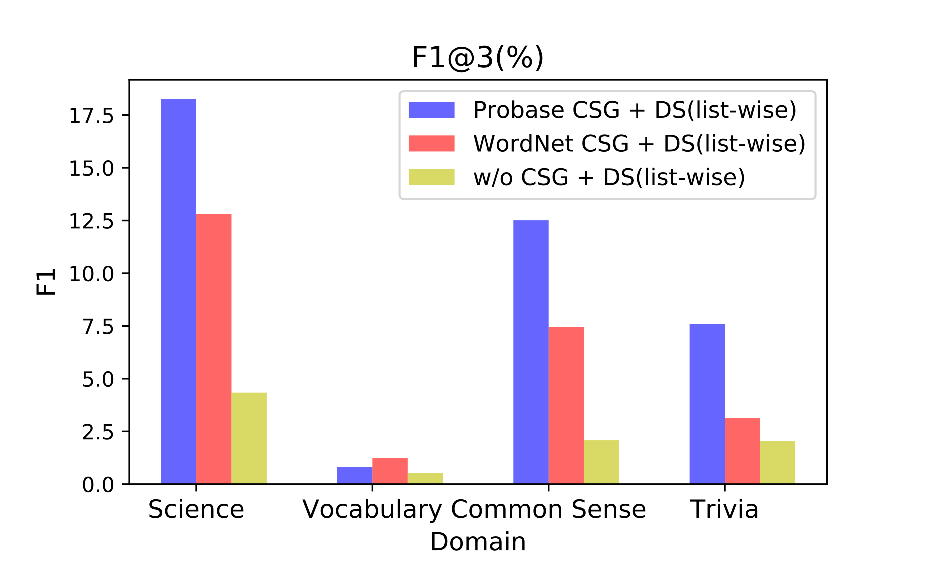
\epsfig{file=figure/f1.eps, width=0.48\columnwidth}
}
% \hfill
\subfloat[Format 2]{
\label{fig:dataset:2}
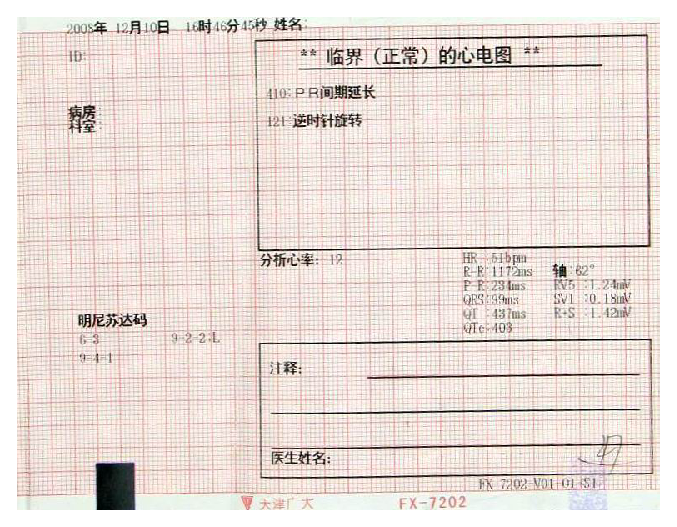
\epsfig{file=figure/f2.eps, width=0.48\columnwidth}
}
\hfill
\subfloat[Format 3]{
\label{fig:dataset:3}
\epsfig{file=figure/f3.eps, width=0.36\columnwidth}
}
\subfloat[Format 4]{
\label{fig:dataset:4}
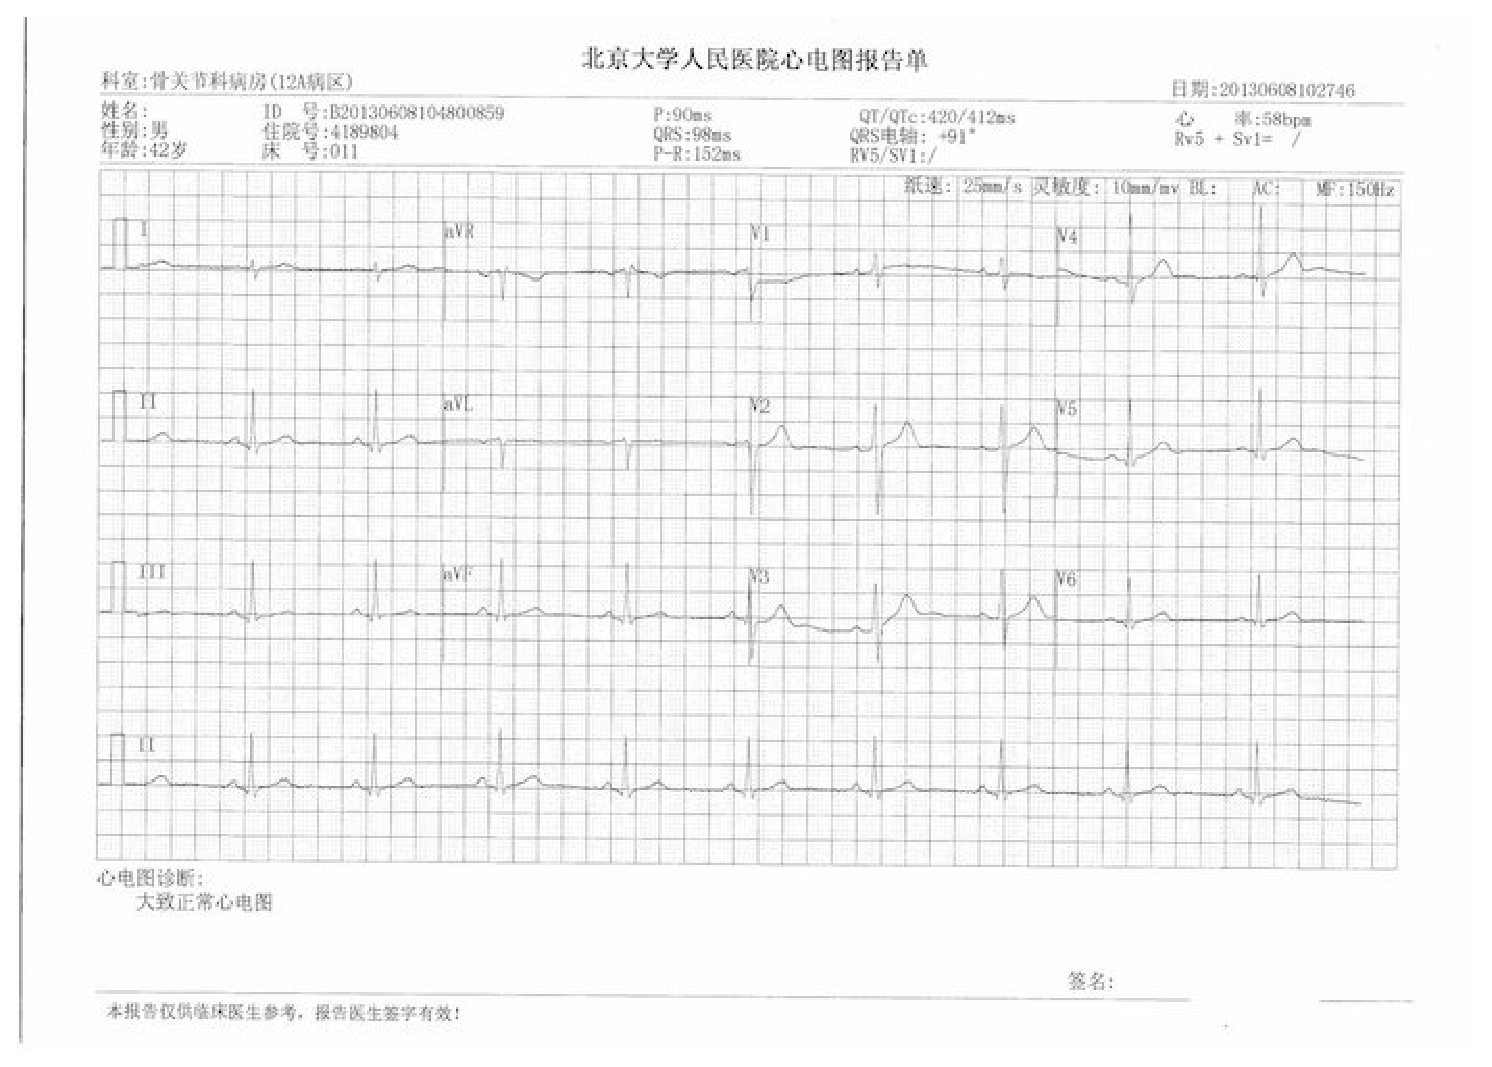
\epsfig{file=figure/f4.eps, width=0.6\columnwidth}
}
\caption{Example images of ECG formats in the dataset.}
\label{fig:dataset}
\end{figure}

\begin{table}[ht]
\centering
\caption{Statistics of the ECG image dataset.}
\label{tab:statis}
%\scalebox{0.5}{
\begin{tabular}{|c|c|c|c|c|}
\hline
Format & 1 & 2 & 3 & 4\\
\hline \hline
Number of Images & 124 & 113 & 102 & 97\\
\hline
Number of Attributes per Image & 17 & 16 & 18 & 15 \\
\hline
\end{tabular}
\end{table}

\paragraph{Image Preprocessing}
The original medical images poses various problems
which affects the performance of the OCR engine.
For example, images are in different colors,
and the textual information are surrounded by grid lines.
To alleviate those problems, we binarize these images
by a simple thresholding approach.
We set separate thresholds for each of the RGB channels of the image,
and combine the output values of all channels with AND operation.
We make use of the auto-thresholding techniques in ImageJ Toolkit \cite{schneider2012nih},
which automatically determine the thresholds and generate the output images.
\figref{fig:preprocess} shows the comparison between the original image
and the corresponding one after preprocessing.
By removing grid lines and turning to a binary image,
the output is much cleaner, making the text on the image stand out.

\begin{figure}[ht]
\centering
\subfloat[Before preprocessing]{
\label{fig:preprocess:1}
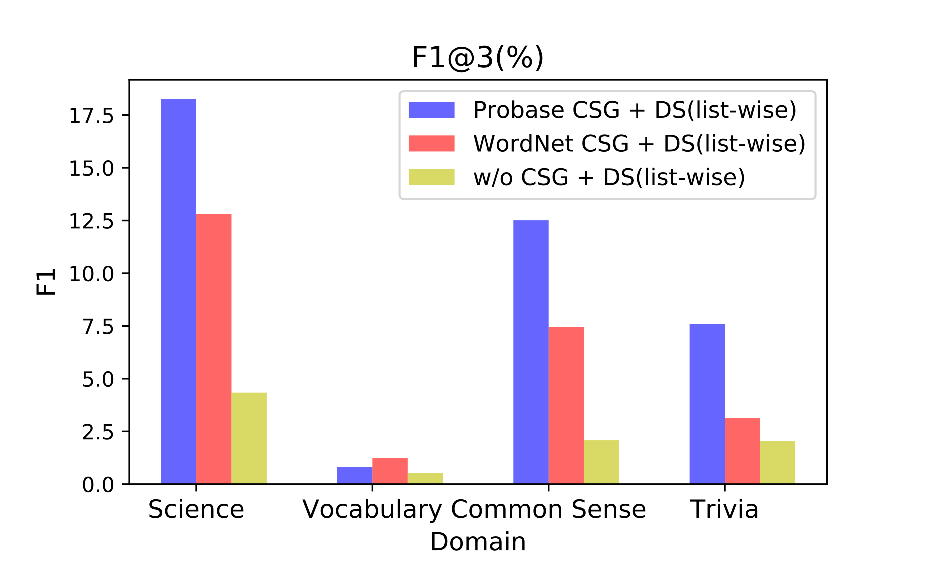
\epsfig{file=figure/f1.eps, width=0.48\columnwidth}
}
\hfill
\subfloat[After preprocessing]{
\label{fig:preprocess:2}
\epsfig{file=figure/preprocess.eps, width=0.48\columnwidth}
}
\caption{Example of image preprocessing.}
\label{fig:preprocess}
\end{figure}


\subsection{Evaluation of Structured Textual Information Extraction}
Now we perform the end-to-end extraction task on
the medical image dataset.
We use the extraction accuracy over variables as the evaluation metric.
For our proposed method (\textit{ODL Parser}),
we adopt Tesseract~\cite{smith2007overview} as the OCR engine.
We split the dataset into 5\% for validation and 95\% for testing.
The hyperparameters $k$, $\tau$ and $w$ are tuned by achieving the
highest accuracy on the validation set.

We compare our method with three competing methods discussed in \secref{sec:intro}.
% the first method is based on a naive zone-of-interest annotation.
% the second method is the improvement of the first one,
% which overcomes the problem brought by xxxx.
The first method (\textit{Exact Match}) is a textual matching approach.
Based on the coordinates of each text box in the raw OCR result,
we restore all text boxes into multiple rows of texts.
Then we write simple regex rules to extract numerical variables
by exactly matching the constant strings before and after them.
No fuzzy matching or data constraints are applied in this method.

The second competing method (\textit{Zonal OCR}) is based on
manually marking zones of each data on the images.
Tesseract is applied for recognizing texts from each image fragment.
%The blue boxes in \figref{fig:zOCR} marks all annotated zones of data.
In order to overcome the slight positional variations between images,
the annotating process is improved in this method.
As shown in \figref{fig:zOCR}, for images of the same format,
we first label all zones of interest in one image (the blue boxes),
as well as another referent zone (the red box).
We keep the relative distance between all boxes,
and only label the referent zone for all the remaining images.
Therefore, all zone of interests of the remaining images
can be automatically calculated.
\begin{figure}[ht]
\centering
\epsfig{file=figure/zonal_OCR.eps, width=0.9\columnwidth}
\caption{Example of ECG image with zones of interests and referent zones.}
\label{fig:zOCR}
\end{figure}

The third approach (\textit{Page Layout}) is based on the page layout analysis,
with examples depicted in \figref{fig:running-page-layout}.
We adopt ABBYY recognizer for page layout analysis,
and implement ad-hoc rules to map the desired data with specific text units
in the page layout result.

% The page layout analysis technique is used to determine where the text
% resides on a page \cite{o1993document}.
% By using the page layout analysis technique, the hierarchy of physical components
% can be generated which we can use to match them to the predefined
% hierarchy of logical components. An example result of our page layout
% analysis is shown in \figref{fig:pl}.
% \begin{figure}[ht]
% \centering
% 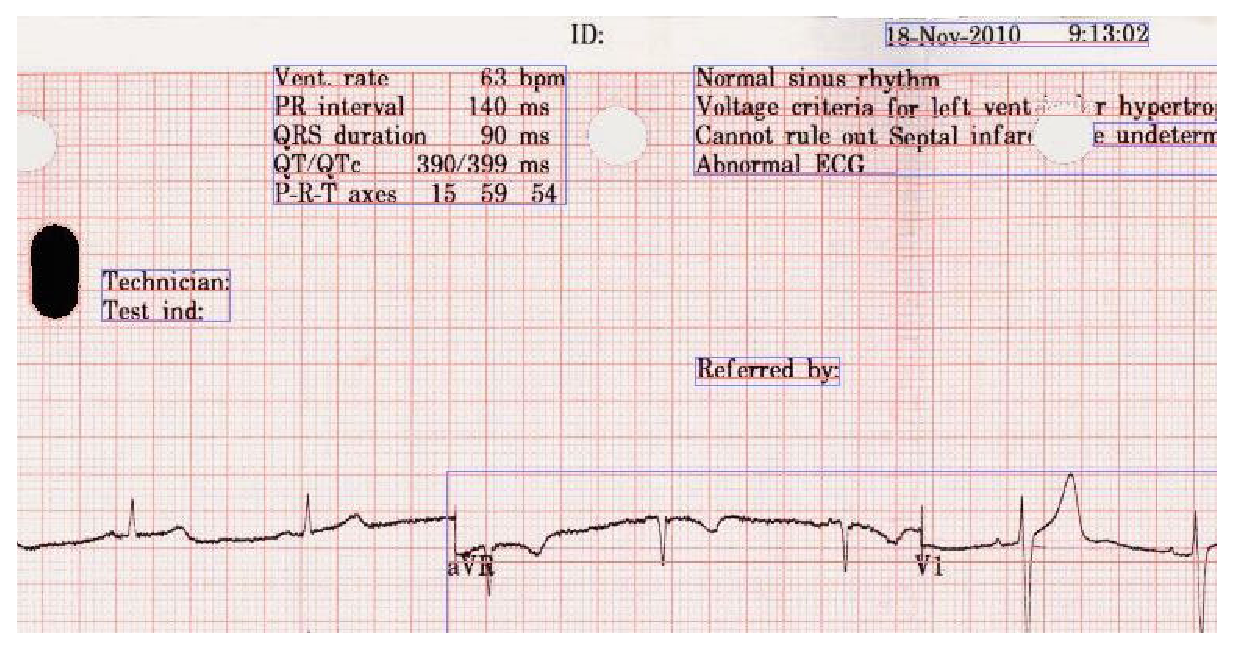
\epsfig{file=figure/17_pl.eps, width=0.8\columnwidth}
% \caption{Example result of page layout analysis.}
% \label{fig:pl}
% \end{figure}


\begin{table}[!hbp]
\centering
\caption{Accuracy of structured information extraction over medical images.}
\label{tab:compare}
\begin{tabular}{|c|c|c|c|c|}
\hline
Format & 1 & 2 & 3 & 4\\
\hline \hline
Exact Match & 58.8\% & 56.3\% & 61.1\% & 53.4\% \\
\hline
Zonal OCR & 81.2\% & 79.8\% & 81.7\% & 80.6\% \\
\hline
Page Layout & 79.7\% & 80.2\% & 81.2\% & 81.1\% \\
\hline
ODL Parser & {\bf 85.5\%} & {\bf 83.8\%} & {\bf 84.9\%} & {\bf 84.0\%}\\
\hline
\end{tabular}
\end{table}

\tabref{tab:compare} shows the experimental results over the testing images.
Our ODL-based approach consistently outperforms existing approaches by
an absolute gain of 3-6\% on all the 4 ECG formats,
which demonstrates the effectiveness of the robust parsing process.
We observe that \textit{Exact Match} baseline is outperformed by the other
approaches by a significant margin,
due to the results are highly affected by noisy text boxes,
as well as the recognition error of either the surrounding constants
or the target variables.
% as the fixed boundary is highly sensitive to
% the problem of slight layout variations.
%Here are reasons for that:
%Zonal OCR's performance will be highly affected by the setting of zones of interest. As for page
%layout analysis, the performance will be affected by the granularity of the page layout unit and the misrecognition will affect the matching with the predefined
%hierarchy of logical components. .
% The performance of
%zonal OCR will be highly affected by the setting of zones of interest.
%If the zones of interest are too large, it's possible that noises will
%also be extracted, while if the zones of interest are too small, results
%can be incomplete. For page layout analysis, the performance will be
%affected by the granularity of the page layout unit and the
%misrecognition will affect the matching with the predefined
%hierarchy of logical components. For our method, the smallest
%unit is word in text so our description can be very accurate.
%At the same time, the fuzzy matching strategies also enable
%the description to omit some unnecessary details.
% \KZ{Need focus on explaining why we are only slightly better, and what are
% the problems of the other three methods, despite that their accuracies are
% not that bad! e.g., efforts to mark the zones, I'm still not convinced
% how come without fuzzy match, zonal methods can be so good since the dist
% between the marker zone and the interesting zones can be slightly off in each
% image.}
The other two baselines,
though marginally outperformed by the ODL-based approach,
still have their own important limitations.
For \textit{Zonal OCR}, the main assumption is that relative layouts of texts
are accurate and unchanged among all the images of the same format.
The assumption makes sense, but doesn't always hold.
%zonal OCR, it's important to adjust the zones of interest based on the marker zone.
Misrecognition of the zone is disastrous,
as all the extracted information will be incorrect.
Besides, the user have to annotate the referent zone for every single image,
which is labour intensive and inefficient.
For \textit{Page Layout},
it also requires the consistent page layout result for images of the same format.
If the textual zone are recognized incorrectly,
necessary information may be omitted from output.
As shown in \figref{fig:errorpl}, the largest textual zone is imperfectly located,
which leads to error information extraction results.
Although having a relative high accuracy,
the extraction wrapper of this method is rather ad-hoc,
which is more challenging for putting into real use.
Compared with those baselines,
the ODL based approach doesn't rely on any carefully defined bounding boxes,
its most important advantage is to make full use of the relative layout
information between expressions embedded in the ODL description.
Based on the implicit layout restrictions,
the parser is able to generate the optimized alignment between
expressions and text boxes, while satisfying both value and spatial constraints.
% However, the fuzzy match design of our system can
% tolerate these types of errors that the OCR engine made.
% We seek to find an optimization solution which can extract
% correct information as much as possible.

\begin{figure}[ht]
\centering
\epsfig{file=figure/error_page_layout.eps, width=0.8\columnwidth}
\caption{Example result of an imperfect page layout analysis.}
\label{fig:errorpl}
\end{figure}


\subsection{Evaluation of Automatic Correction}
%In this section, we compare the performance of
%the human correction part in our system.
%Another important part of our system is the human correction
%process. By making use of the human power, we can correct
%the errors that occur due to the OCR engine.
In this section, we conduct the additional experiments to
analyze the performance gain brought by human correction in our system.
For each image format, the system prompts a certain number of
imperfect $(e, d.text)$ alignments as parsing errors,
collects all manual correction data,
and performs a new run of parsing based on the updated correction model.
Given the set of all detected parsing errors,
we compare two policies of recommending errors for manual correction:
\textit{random} and \textit{most frequent}.
For the \textit{random} policy,
the system follows the 2-step sampling without replacement:
first randomly samples $e$ from all distinct expressions with parsing errors,
then randomly selects one instance from all parsing errors related to $e$.
The \textit{most frequent} policy is also based on sampling without replacement,
while for each pick,
the system always randomly samples the parsing error from those expressions
with the most parsing errors.
% the system focus on the top-3 expressions with the most parsing errors,
% then uniformly samples parsing errors from them. \KZ{What do you mean by
% ``focus''? Uniform sample means pick one randomly from the 3?
% This is a bit unnatural. Why not just pick the top-1?}

\figref{fig:humancorr} reports the extraction accuracies
with 0, 1, 5, 10, 15 human corrections using different recommending policies.
For each specification, we conduct the experiment 100 times,
and report the average accuracy.
Due to the intensive labour in repeating experiments,
we didn't perform experiments on larger human corrections.
For all different image formats, the more corrections we make,
the better accuracy we can get,
which demonstrates the effectiveness of the correction model.
The improvement to the extraction accuracy is better when using the
\textit{most frequent} policy instead of the \textit{random} baseline.
We argue that by paying more attentions to the most common recognitions errors,
the correction model under the \textit{most frequent} recommendation
is able to correct more imperfect alignments,
rather than wasting limited corrections to long-tail cases.
In addition, for the accuracy curve of the \textit{most frequent} policy,
we observe that the growing rate goes down when increasing the number of
human corrections.
This is reasonable, as compared with frequent recognitions errors,
the incremental corrections on infrequent ones lead to fewer improvements.


% recommendation because using the most
% frequent recommendation is more efficient in making use of human judgment.
% We also find that with more corrections made, the improvement of
% accuracy tends to saturate, especially with regard to the most frequent error strategy.
%
% The reason is that, based on our learning model,
% our system tends to get less useful information
% from the correction. The corrections that will affect
% the whole system should be made early, so
% unusable corrections will be left.
% \KZ{Need to explain why there's only limited improvement after 15 corrections.
% Maybe because the data size is not big enough, so there's not many repeated
% errors?}
% The growing rate of accuracies goes down when increasing the number of human corrections.
%
% The improvement of accuracy is limited after 15 corrections.
% The main reason is that there are not many repeated errors due to
% the small size of the data set and furthermore, our system can only make corrections
% according to the correction model, which is sensitive to such errors.


\begin{figure*}[ht]
\centering
\subfloat{
%% \label{fig:hc:1}
\epsfig{file=figure/hcf1.eps, width=0.48\columnwidth}
}
% \hfill
% \centering
\subfloat{
% \label{fig:hc:2}
\epsfig{file=figure/hcf2.eps, width=0.48\columnwidth}
}
\hfill
% % \centering
\subfloat{
% \label{fig:hc:3}
\epsfig{file=figure/hcf3.eps, width=0.48\columnwidth}
}
% % \centering
\subfloat{
% \label{fig:hc:4}
\epsfig{file=figure/hcf4.eps, width=0.48\columnwidth}
}
\caption{Extraction accuracy with human annotated correction.}
\label{fig:humancorr}
\end{figure*}

% \begin{enumerate}
% \item Compare the description code with generated code to show our language is a simple one;
% \item Compare the accuracy with baseline, exact match on the OCR results, to show our language can tolerate the noises and errors;
% \item Compare the performance on different image formats;

% \item Compare the accuracy between our approach and others, including using related image position;

% TODO: really need the discussion here?
% Although our system achieves good results based on our
% experiments, there are some limitations that call for future
% work. First, we need to provide enough constraints in the description.
% %such as the type of the
% %data or the range of the data.
% If the constraints are not
% sufficiently specified, it is hard for our system to evaluate what
% data among the OCR outputs are more suitable for the description.
% For example, if we constrain the data to be an integer in the
% description, then any integers that appear in the OCR output can be
% candidates if they satisfy the spatial constraints.
% %In many cases, insufficiency in the constraints can be
% %made up by the constraints indicated from the neighboring descriptions.
% %But sometimes, simple descriptions will lead to sub-standard results.
% Second, the correction model
% we generated is a probabilistic model based on the statistics.
% This correction model can make mistakes,
% e.g., correcting the right answer into the wrong one. More data
% from manual correction will help to reduce this possibility.
%
% % \KZ{Perhaps there's more issues you can discuss, now that u have
% % changed the def of the correction model...}
